%%%%%%%%%%%%%%%%%%%%%%%%%%%%%%%%%%%%%%%%%%
%%%%%%%%%%%%%                 %%%%%%%%%%%%
%%%%%%%%%%%%%    EXERCISE 1   %%%%%%%%%%%%
%%%%%%%%%%%%%                 %%%%%%%%%%%%
%%%%%%%%%%%%%%%%%%%%%%%%%%%%%%%%%%%%%%%%%%
\begin{exercise}[Capacity of the carrier pigeon channel]{Consider a commander of an army besieged in a fort for whom the only means of communication to his allies is a set of carrier pigeons. Assume that each carrier pigeon can carry one letter (8 bits), that pigeons are released once every 5 minutes, and that each pigeon takes exactly 3 minutes to reach its destination.
  \begin{enumerate}
    \item Assuming that all the pigeons reach safely, what is the capacity of this link in bits/hour?
    \item Now assume that the enemies try to shoot down the pigeons and that they manage to hit a fraction $\alpha$ of them. since the pigeons are sent at a constant rate, the receiver knows when the pigeons are missing. What is the capacity of this link?
    \item Now assume that the enemy is more cunning and that every time they shoot down a pigeon, they send out a dummy pigeon carrying a random letter (chosen uniformly from all 8-bit letters). What is the capacity of this link in bits/hour? Set up an appropriate model for the channel in each of the above cases, and indicate how to go about finding the capacity.
  \end{enumerate}}
  \begin{solution}
  \par{~}
  \begin{enumerate}
    \item { The capacity is 8 bits/5mins $=$ 96 bits/hour.
    }
    \item { The process can be modeled as an erasure model. Consider the transmission of a pigeon of 8 bits (256 alphabets), it has the probability of $\alpha$ to be erased. We assume the message sent is $X \in \left\{0, \ldots, 256 \right\}$, the message received is $Y \in \left\{e, 0, \ldots, 256\right\}$. The capacity of a single transmission is
    \begin{equation}
      \begin{aligned}
        C &=\max _{p(x)} I(X ; Y) \\
        &=\max _{p(x)}(H(Y)-H(Y | X))\\
        &=\max _{p(x)} (H(Y)-H(\alpha)) \\
        &=\max _{\pi}((1-\alpha) H(Y|X = Y)+H(\alpha)-H(\alpha))\\
        &=\log(256) (1- \alpha)
      \end{aligned}
    \end{equation}  
    Hence the capacity is $8(1-\alpha)$ bits per pigeon, or $96(1-\alpha)$ bits per hour.
    }
    \item { The process can be modeled as a binary symmetric channel. Consider the transmission of a pigeon of 8 bits (256 alphabets), it has the probability of $\frac{\alpha}{256}$ to be changed to a different value. We assume the message sent is $X \in \left\{0, \ldots, 256 \right\}$, the message received is $Y \in \left\{0, \ldots, 256\right\}$. The capacity of a single transmission is
    \begin{equation}
      \begin{aligned}
        C&=\max I(X ; Y) \\
 &=\max H(Y)-H(Y | X) \\
 &=\max H(Y)-\sum p(x) H(Y | X=x) \\
 &=\max H(Y)-H\left(1 - \frac{255\alpha}{256}, \frac{\alpha}{256}, \ldots, \frac{\alpha}{256}\right) \\
 &= 16 + \frac{255}{256}\alpha \log \frac{256-255\alpha}{\alpha} - \log (256 - 255\alpha) 
        \end{aligned}
    \end{equation}  
    Hence the capacity is $16 + \frac{255}{256}\alpha \log \frac{256-255\alpha}{\alpha} - \log (256 - 255\alpha)$ bits per pigeon, or $12(16 + \frac{255}{256}\alpha \log \frac{256-255\alpha}{\alpha} - \log (256 - 255\alpha))$ bits per hour.
    
    }
  \end{enumerate}
  \end{solution}
  \label{ex7-1}
\end{exercise}

%%%%%%%%%%%%%%%%%%%%%%%%%%%%%%%%%%%%%%%%%%
%%%%%%%%%%%%%                 %%%%%%%%%%%%
%%%%%%%%%%%%%    EXERCISE 2   %%%%%%%%%%%%
%%%%%%%%%%%%%                 %%%%%%%%%%%%
%%%%%%%%%%%%%%%%%%%%%%%%%%%%%%%%%%%%%%%%%%
\begin{exercise}[Channel with two independent looks at $Y$]{ Let $Y_{1}$ and $Y_{2}$ be conditionally independent and conditionally identically distributed given
  $X$
  \begin{enumerate}
    \item Show that $I\left(X ; Y_{1}, Y_{2}\right)=2 I\left(X ; Y_{1}\right)-I\left(Y_{1}, Y_{2}\right)$
    \item Conclude that the capacity of the channel $(X\mapsto Y_1,Y_2)$ is less than twice the capacity of channel $(X \mapsto Y_1)$
  \end{enumerate} }
  \begin{proof}
  \par{~}
  \begin{enumerate}
    \item {
      \begin{equation}
        \begin{aligned}
          I(X;Y_1,Y_2) &= H(Y_1,Y_2) - H(Y_1,Y_2|X) \\
          &= H(Y_1,Y_2) - H(Y_1|X) - H(Y_2|X) \\
          &= H(Y_1) + H(Y_2) - I(Y_1;Y_2) -  H(Y_1|X) - H(Y_2|X) \\
          &=I(X;Y_1) + I(X;Y_2)- I(Y_1,Y_2) \\
          &= 2I(X;Y_1) - I(Y_1,Y_2)
        \end{aligned}
      \end{equation}
     }
    \item { 
\begin{equation}
  \begin{aligned}
    C_1 &= \max_{p(x)} I(X;Y_1,Y_2) \\
    &= \max_{p(x)} (2I(X;Y_1) - I(Y_1,Y_2)) \\
    &\le \max_{p(x)} 2I(X;Y_1) \\
    &= 2C_2
  \end{aligned}
\end{equation}
    }
  \end{enumerate}
  \end{proof}
  \label{ex7-2}
\end{exercise}

%%%%%%%%%%%%%%%%%%%%%%%%%%%%%%%%%%%%%%%%%%
%%%%%%%%%%%%%                 %%%%%%%%%%%%
%%%%%%%%%%%%%    EXERCISE 3   %%%%%%%%%%%%
%%%%%%%%%%%%%                 %%%%%%%%%%%%
%%%%%%%%%%%%%%%%%%%%%%%%%%%%%%%%%%%%%%%%%%
\begin{exercise}[Binary multiplier channel]{\par{~}
  \begin{enumerate}
    \item Consider the channel $Y=X Z$, where $X$ and $Z$ are independent binary random variables that take on values 0 and $1 . Z$ is Bernoulli($\alpha \text {) [i.e., } P(Z=1)=\alpha] .$ Find the capacity of this channel and the maximizing distribution on $X$.
    \item Now suppose that the receiver can observe $Z$ as well as $Y$. What is the capacity?
  \end{enumerate} }
  \begin{solution}
  \par{~}
  \begin{enumerate}
    \item { Let $p(X=1)= \pi$
    \begin{equation}
      \begin{aligned}
        I(Y;X) &= H(Y) - H(Y|X) \\
        &= H(\alpha \pi) - \pi H(\alpha) \\
        &= - \alpha\pi \log \alpha\pi - (1 - \alpha\pi) \log (1- \alpha\pi) - H(\alpha)\pi
       \end{aligned}
    \end{equation}
    We find the maximal value by taking the derivative.
    \begin{equation}
      \begin{aligned}
        \frac{dI(Y;X)}{d\pi} &= - \alpha \log \alpha\pi - \frac{\alpha}{\ln 2} + \alpha \log (1-\alpha \pi) + \frac{\alpha}{\ln 2} - H(\alpha) \\
        &= \alpha \log \frac{1-\alpha\pi}{\alpha\pi} - H(\alpha) := 0 \\
        \frac{1-\alpha\pi}{\alpha\pi} &= 2^{\frac{H(\alpha)}{\alpha}} \\
        \pi^{*} &= \frac{1}{\alpha\left(2^{\frac{H(\alpha)}{\alpha}}+1\right)} \\
        C &= \log \left(2^{\frac{H(\alpha)}{\alpha}}+1\right)-\frac{H(\alpha)}{\alpha}
      \end{aligned}
    \end{equation}
    }
    \item { Let $p(X=1)= \pi$
    \begin{equation}
      \begin{aligned}
        I(Y,Z;X) &= H(Y,Z) - H(Y,Z|X) \\
        &= H(Y|Z) + H(Z) - H(Y|Z,X) - H(Z|X) \\
        &= H(Y|Z) - H(XZ|Z,X) = H(XZ|Z) \\
        &= \alpha H(\pi) \le \alpha
       \end{aligned}
    \end{equation}
    The maximal value is obtained when $X$ is normally distributed.
    }
  \end{enumerate}
  \end{solution}
  \label{ex7-3}
\end{exercise}

%%%%%%%%%%%%%%%%%%%%%%%%%%%%%%%%%%%%%%%%%%
%%%%%%%%%%%%%                 %%%%%%%%%%%%
%%%%%%%%%%%%%    EXERCISE 4   %%%%%%%%%%%%
%%%%%%%%%%%%%                 %%%%%%%%%%%%
%%%%%%%%%%%%%%%%%%%%%%%%%%%%%%%%%%%%%%%%%%
\begin{exercise}[Noise Channel]{Consider the channel $\mathcal{X}=\{0,1,2,3\},$ where $Y=X+Z,$ and $Z$ is uniformly distributed over three distinct integer values $\mathcal{Z}=\left\{z_{1}, z_{2}, z_{3}\right\}$
  \begin{enumerate}
    \item What is the maximum capacity over all choices of the $\mathcal{Z}$ alphabet? Give distinct integer values $z_{1}, z_{2}, z_{3}$ and a distribution on     $\mathcal{X}$ achieving this.
    \item What is the minimum capacity over all choices for the $\mathcal{Z}$ alphabet? Give distinct integer values $z_{1}, z_{2}, z_{3}$ and a distribution on
    $\mathcal{X}$ achieving this.
  \end{enumerate} }
  \begin{solution}
  \par{~}
  \begin{enumerate}
    \item { 
    \begin{equation}
      \begin{aligned}
        I(Y;X) &= H(X) - H(X|X+Z) \\
        &\le H(x)  \le \log 4 = 2
      \end{aligned}
    \end{equation}  
    The maximal capacity will be achieved when $X$ is a function of $Y$, i.e. given $Y$, $X$ can be determined, and that $X$ is normally distributed. A choice of $\mathcal{Z}$ can be $\mathcal{Z}=\left\{0, 5, 10 \right\}$ }
    \item {
      \begin{equation}
        \begin{aligned}
          I(Y;X) &= H(Y) - H(X+Z|X) = H(X+Z) - H(Z) \\
          &= H(X+Z) - \log 3 
        \end{aligned}
      \end{equation}
      Note that for any single possible $X$, there will be at most 3 distinct corresponding $Y$. In order to minimize the maximal $H(X+Z)$, we need to set $Z$ to be 3 continuous numbers, so that the uncertainty of $X+Z$ will be minimized. We take $\mathcal{Z}=\left\{0, 1, 2 \right\}$ for example. Let the distribution of $\mathcal{X}$ to be $\left\{p_1, p_2, p_3,p_4 \right\}$ Then
      \begin{equation}
          H(X+Z) = H(\frac{p_1}{3}, \frac{p_1 + p_2}{3}, \frac{p_1+p_2+p_3}{3}, \frac{p_2+p_3+p_4}{3}, \frac{p_3+p_4}{3}, \frac{p_4}{3}) \le \log 6
      \end{equation}
      The maximal value is obtained when $p_1 = p_4 =  \frac{1}{2}$. Hence the channel capacity is 1.
     }
  \end{enumerate}
  \end{solution}
  \label{ex7-4}
\end{exercise}

%%%%%%%%%%%%%%%%%%%%%%%%%%%%%%%%%%%%%%%%%%
%%%%%%%%%%%%%                 %%%%%%%%%%%%
%%%%%%%%%%%%%    EXERCISE 5   %%%%%%%%%%%%
%%%%%%%%%%%%%                 %%%%%%%%%%%%
%%%%%%%%%%%%%%%%%%%%%%%%%%%%%%%%%%%%%%%%%%
\begin{exercise}[Erasure channel.]{Let $\{\mathcal{X}, p(y | x), \mathcal{Y}\}$ be a discrete memoryless channel with capacity $C$. Suppose that this channel is cascaded immediately with an erasure channel $\{\mathcal{Y}, p(s | y), \mathcal{S}\}$ that erases $\alpha$ of its symbols. Specifically, $\mathcal{S}=\left\{y_{1}, y_{2}, \ldots, y_{m}, e\right\},$ and
  $$
  \begin{array}{ll}
  \operatorname{Pr}\{S=y | X=x\}=\bar{\alpha} p(y | x), & y \in \mathcal{Y} \\
  \operatorname{Pr}\{S=e | X=x\}=\alpha
  \end{array}
  $$
  Determine the capacity of this channel.
  \begin{figure}[H]
    \centering
    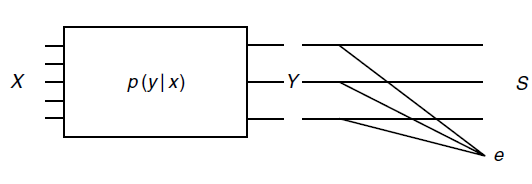
\includegraphics[height=4cm]{img/7-1.png}
    \caption{Erasure Channel}
    \label{fig:ex5}
  \end{figure}
  }
  \begin{solution}
  \begin{equation}
    \begin{aligned}
      I(X;S) &= H(S) -H(S|X) \\
      &= H(S) - \sum_{x\in\mathcal{X}} p(x) \left( \left(\sum_{y\in\mathcal{Y}} \bar{\alpha} p(y|x) \log \bar{\alpha} p(y|x)\right) - \alpha \log \alpha \right) \\
      &= H(S) - \sum_{x\in\mathcal{X}} p(x) \left(\sum_{y\in\mathcal{Y}} \bar{\alpha} p(y|x) \left( \log \bar{\alpha} + \log p(y|x) \right)\right) - \alpha \log \alpha  \\
      &= H(S) - \sum_{x\in\mathcal{X}} p(x) \sum_{y\in\mathcal{Y}} \bar{\alpha} p(y|x)  \log p(y|x) - \alpha \log \alpha - \bar{\alpha} \log \bar{\alpha} \\
      &= H(S) - H(\alpha) -  (1-\alpha) H(Y|X) \\
      &= - \sum_{y\in\mathcal{Y}} \bar{\alpha}p(y) \log \bar{\alpha}p(y) - \alpha\log\alpha - H(\alpha) -  (1-\alpha) H(Y|X) \\
      &= - \sum_{y\in\mathcal{Y}} \bar{\alpha}p(y) \left( \log \bar{\alpha} + \log p(y) \right)  - \alpha\log\alpha - H(\alpha) -  (1-\alpha) H(Y|X) \\
      &= - \sum_{y\in\mathcal{Y}} \bar{\alpha} p(y)  \log p(y) -\bar{\alpha}\log\bar{\alpha} - \alpha\log\alpha - H(\alpha) -  (1-\alpha) H(Y|X) \\
      &= (1-\alpha) H(Y) + H(\alpha)  - H(\alpha)  -  (1-\alpha) H(Y|X)  \\
      &= (1-\alpha) I(X;Y)
    \end{aligned}
  \end{equation}
  Therefore the capacity of this channel is $(1-\alpha)C$.
  \end{solution}
  \label{ex7-5}
\end{exercise}

%%%%%%%%%%%%%%%%%%%%%%%%%%%%%%%%%%%%%%%%%%
%%%%%%%%%%%%%                 %%%%%%%%%%%%
%%%%%%%%%%%%%    EXERCISE 6   %%%%%%%%%%%%
%%%%%%%%%%%%%                 %%%%%%%%%%%%
%%%%%%%%%%%%%%%%%%%%%%%%%%%%%%%%%%%%%%%%%%
\begin{exercise}[Choice of channels]{Find the capacity $C$ of the union of two channels $\left(\mathcal{X}_{1}, p_{1}\left(y_{1} | x_{1}\right), \mathcal{Y}_{1}\right)$ and $\left(\mathcal{X}_{2},\right.$ $\left. p_{2}\left(y_{2} | x_{2}\right), \mathcal{Y}_{2}\right),$ where at each   time, one can send a symbol over channel 1 or channel 2 but not both. Assume that the output alphabets are distinct and do not intersect.
  \begin{enumerate}
    \item Show that $2^{C}=2^{C_{1}}+2^{C_{2}} .$ Thus, $2^{C}$ is the effective alphabet size of a channel with capacity $C$
    \item Compare with Problem 2.10 where $2^{H}=2^{H_{1}}+2^{H_{2}}$, and interpret part (a) in terms of the effective number of noise-free symbols.
    \item Use the above result to calculate the capacity of the following channel.
  \end{enumerate}
  \begin{figure}[H]
    \centering
    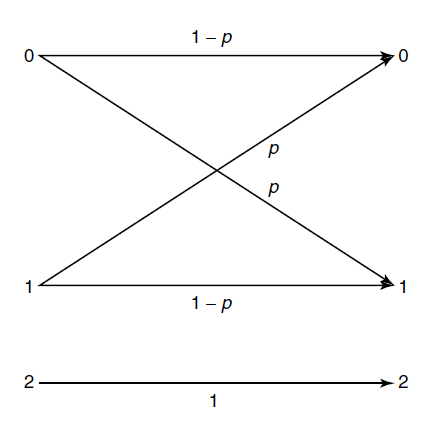
\includegraphics[height=6cm]{img/7-2.png}
    \caption{Choice of Channels}
    \label{fig:ex6}
  \end{figure}
  
  }
  \begin{solution}
  \par{~}
  \begin{enumerate}
    \item { We assume
    \begin{equation}
      p(X=x) = \left\{ \begin{array}{l}
        \pi, x=X_1 \\
        1-\pi, x=X_2
      \end{array}\right.
    \end{equation}
    \begin{equation}
      \begin{aligned}
        I(X,Y) &= H(X) - H(X|Y) \\
        &= - \sum_{x\in \mathcal{X_1 \cup X_2}} p_{X}(x)\log p_{X}(x) - \pi H(X_1|Y_1) - \bar{\pi}H(X_2|Y_2) \\
        &= - \sum_{x\in \mathcal{X_1}} \pi p_{X_1}(x) \log \pi p_{X_1}(x) - \sum_{x\in \mathcal{X_2}} \bar{\pi} p_{X_2}(x) \log \bar{\pi} p_{X_2}(x)  - \pi H(X_1|Y_1) - \bar{\pi}H(X_2|Y_2) \\
        &= H(\pi) + \pi H(X_1) + \bar{\pi} H(X_2) - - \pi H(X_1|Y_1) - \bar{\pi}H(X_2|Y_2) \\
        &= H(\pi) + \pi I(X_1;Y_1) + \bar{\pi} I(X_2;Y_2) \\
        &\le H(\pi) + \pi C_1  + \bar{\pi} C_2
      \end{aligned}
    \end{equation}
    The equality holds when $p(x_1)$ and $p(x_2)$ are at their optimal distribution. We take the derivative on $\pi$ to calculate the capacity.
    \begin{equation}
      \begin{aligned}
        \frac{dI(X;Y)}{d\pi} &= - \log \pi + \log (1-\pi) + C_1 - C_2 := 0\\
        \frac{\pi^{*}}{1-\pi^{*}} &= 2^{C_1-C_2} \\
        \pi^{*} &= \frac{2^{C_1}}{2^{C_1}+2^{C_2}} \\
        \Rightarrow C &= \log (2^{C_1}+2^{C_2})
      \end{aligned}
    \end{equation}
    It follows that $2^C = 2^{C_1} + 2^{C_2}$
    }
    \item { Using the same notion as Assignment3.7, $2^C$ is the effective number of noise-free symbols. Since the two channels are disjoint in their alphabets, the noise-free symbols will also not overlap. Hence the combined capacity is equal to the sum of two sub-channels' noise-free symbols, i.e.  $2^C = 2^{C_1} + 2^{C_2}$}
    \item { From the Binary Symmetric Channel we know that $C_1 = 1 - H(p)$. $C_2 = 0$. Hence we have $C = \log (2^{1-H(p)} +1)$
    }
  \end{enumerate}
  \end{solution}
  \label{ex7-6}
\end{exercise}

%%%%%%%%%%%%%%%%%%%%%%%%%%%%%%%%%%%%%%%%%%
%%%%%%%%%%%%%                 %%%%%%%%%%%%
%%%%%%%%%%%%%    EXERCISE 7   %%%%%%%%%%%%
%%%%%%%%%%%%%                 %%%%%%%%%%%%
%%%%%%%%%%%%%%%%%%%%%%%%%%%%%%%%%%%%%%%%%%
\begin{exercise}[Capacity]{Suppose that channel $\mathcal{P}$ has capacity $C,$ where $\mathcal{P}$ is $m \times n$ channel matrix.
  \begin{enumerate}
    \item What is the capacity of
    $$
    \tilde{\mathcal{P}}=\left[\begin{array}{ll}
    \mathcal{P} & 0 \\
    0 & 1
    \end{array}\right] ?
    $$
    \item  What about the capacity of
    $$
    \hat{\mathcal{P}}=\left[\begin{array}{cc}
    \mathcal{P} & 0 \\
    0 & I_{k}
    \end{array}\right] ?
    $$
    where $I_{k}$ if the $k \times k$ identity matrix.
  \end{enumerate} }
  \begin{solution}
  \par{~}
  \begin{enumerate}
    \item { Note that the new channel is composed of two disjoint sub-channels, $\mathcal{P}$ and a one-to-one channel whose capacity is $1$. By the conclusion of Exercise \ref{ex7-6}, we know that $C_{\mathcal{P}} = \log (2^{C} + 2^{0}) = \log (2^{C} + 1)$. }
    \item { Note that the new channel is composed of two disjoint sub-channels, $\mathcal{P}$ and a one-to-one channel whose capacity is $\log k$. By the conclusion of Exercise \ref{ex7-6}, we know that $C_{\mathcal{P}} = \log (2^{C} + 2^{\log k}) = \log (2^{C} + k)$. }
  \end{enumerate}
  \end{solution}
  \label{ex7-7}
\end{exercise}

%%%%%%%%%%%%%%%%%%%%%%%%%%%%%%%%%%%%%%%%%%
%%%%%%%%%%%%%                 %%%%%%%%%%%%
%%%%%%%%%%%%%    EXERCISE 8   %%%%%%%%%%%%
%%%%%%%%%%%%%                 %%%%%%%%%%%%
%%%%%%%%%%%%%%%%%%%%%%%%%%%%%%%%%%%%%%%%%%
\begin{exercise}[Channel with memory]{ Consider the discrete memoryless channel $Y_{i}=Z_{i} X_{i}$ with input alphabet $X_{i} \in\{-1,1\}$
  \begin{enumerate}
    \item What is the capacity of this channel when $\left\{Z_{i}\right\}$ is i.i.d. with
    $$
    Z_{i}=\left\{\begin{aligned}
    1, & p=0.5 \\
    -1, & p=0.5 ?
    \end{aligned}\right.
    $$
    Now consider the channel with memory. Before transmission begins, $Z$ is randomly chosen and fixed for all time. Thus, $Y_{i}=Z X_{i}$
    \item  What is the capacity if
    $$
    Z=\left\{\begin{aligned}
    1, & p=0.5 \\
    -1, & p=0.5 ?
    \end{aligned}\right.
    $$
  \end{enumerate}  }
  \begin{solution}
  \par{~}
  \begin{enumerate}
    \item { The channel can be modeled as a binary symmetric channel with false rate 0.5, hence the capacity is $1-H(0.5) = 0$.}
    \item { Since $Z$ is fixed for all time, we can set $X_0$ to be 1, and use $Y_i$ to determine what $Z$ is. Then for the rest of the transmissions, $Y$ becomes a function of $X$. Therefore the capacity will approach $\log |\mathcal{X}| = 1$ as $n \rightarrow \infty$. }
  \end{enumerate}
  \end{solution}
  \label{ex7-8}
\end{exercise}

%%%%%%%%%%%%%%%%%%%%%%%%%%%%%%%%%%%%%%%%%%
%%%%%%%%%%%%%                 %%%%%%%%%%%%
%%%%%%%%%%%%%    EXERCISE 9   %%%%%%%%%%%%
%%%%%%%%%%%%%                 %%%%%%%%%%%%
%%%%%%%%%%%%%%%%%%%%%%%%%%%%%%%%%%%%%%%%%%
\begin{exercise}[Tall, fat people]{Suppose that the average height of people in a room is 5 feet. Suppose that the average weight is 100 lb.
  \begin{enumerate}
    \item Argue that no more than one-third of the population is 15 feet tall.
    \item Find an upper bound on the fraction of 300 -Ib 10 -footers in the room.
  \end{enumerate} }
  \begin{solution}
  \par{~}
  \begin{enumerate}
    \item { The height of people can be regarded as a random variable $X$. By Markov’s inequality,
    $$\operatorname{Pr}\{X \geq 15\} \leq \frac{5}{15} = \frac{1}{3}$$
    }
    \item { The weight of people can be regarded as a random variable $Y$. By Markov’s inequality,
    $$\operatorname{Pr}\{Y \geq 300\} \leq \frac{100}{300} = \frac{1}{3}$$}
    and that
    $$\operatorname{Pr}\{X \geq 10\} \leq \frac{5}{10} = \frac{1}{2}$$
    Hence there are at most $\frac{1}{3}$ 300-lb, 10-footers among all the people.
  \end{enumerate}
  \end{solution}
  \label{ex7-9}
\end{exercise}